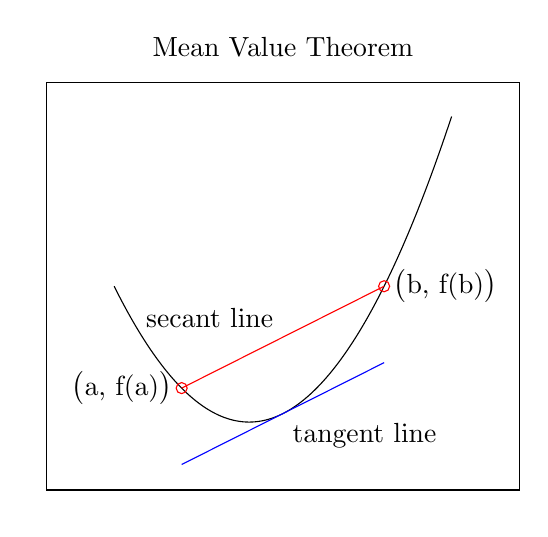
\begin{tikzpicture}
			\begin{axis}[
					scale only axis,
					width  = 6cm,
					xmin   = -1.5,
					xmax   = 2,
					ymin   = -0.5,
					ymax   = 2.5,
					xtick  = \empty,
					ytick  = \empty,
					xlabel = \empty,
					ylabel = \empty,
					title  = Mean Value Theorem,
					smooth,
				]

				% secant and tangent lines
				\addplot[
					domain  = -1:1.5,
					samples = 1000,
				]{x^2};

				\addplot[
					color = red,
					mark  = o,
				] coordinates {(-0.5, 0.25)(1,1)};

				\addplot[
					color = blue,
					mark  = none,
				] coordinates {(-0.5, -5/16) (1, 7/16)};

				% Labels
				\node[left] at (-0.5, 0.25) {\big(a, f(a)\big)};
				\node[right] at (1, 1) {\big(b, f(b)\big)};
				\node[above left] at (0.25, 0.625) {secant line};
				\node[below right] at (1/4, 1/16) {tangent line};
			\end{axis}
		\end{tikzpicture}
